%
% teil2.tex -- Beispiel-File für teil2 
%
% (c) 2020 Prof Dr Andreas Müller, Hochschule Rapperswil
%
% !TEX root = ../../buch.tex
% !TEX encoding = UTF-8
%

\section{Optimierung der Aufstiegsgeschwindigkeit und Geschwindigkeitsverluste \label{leo:section:aufstiegsgleichung}}
\kopfrechts{Optimierung der Aufstiegsgeschwindigkeit}

Die optimale Flugbahn einer Rakete während des Aufstiegs ist entscheidend, um den Treibstoffverbrauch zu minimieren und die Endgeschwindigkeit zu maximieren. 
Die Verluste entstehen hauptsächlich durch Luftwiderstand, Steuerung und Schwerkraft. 
Diese Verluste beeinflussen den erreichbaren Geschwindigkeitszuwachs und damit die Endgeschwindigkeit der Rakete, die am Ende des Aufstiegs benötigt wird, um in den Orbit zu gelangen. 
Eine vereinfachte Formel, die diese Verluste berücksichtigt, ist

\begin{equation}
	v_f = \underbrace{v_* \ln \left(\frac{m_0}{m_f}\right)}_{\text{Raketengleichung}} 
	- \underbrace{2F_* \int_0^{t_f} \frac{\sin^2\left(\frac{\alpha}{2}\right)}{m} \, dt }_{\text{Steuerverluste}}
	- \underbrace{\frac{1}{H} \int_0^{t_f} k_Dv^2 e^{-\frac{h}{H}} \, dt }_{\text{Strömungsverluste}}
	- \underbrace{\int_0^{t_f} g \sin \left(\gamma\right) \, dt}_{\text{Schwerkraftverluste}}.
	\label{leo:aufstiegsgleichung}
\end{equation}

Diese Gleichung fasst die verschiedenen Verluste zusammen, die den erreichbaren Geschwindigkeitszuwachs während des Aufstiegs einschränken. 
Die einzelnen Komponenten werden im Folgenden erklärt.

\subsection{Raketengleichung \label{leo:section:raketengleichung}}
Ein Raumfahrzeug, das sich in einem Orbit um einen Planeten bewegt, verhält sich ähnlich wie ein Gegenstand, der an einem Seil im Kreis geschwungen wird. 
Die notwendige Geschwindigkeit, damit ein Raumfahrzeug in einer stabilen Umlaufbahn bleibt, wird durch die Gleichung
\[
v = \sqrt{\frac{\mu}{r}}
\]
beschrieben, wobei \(r\) der Abstand vom Mittelpunkt des Planeten zur Rakete und \(\mu\) der Gravitationsparameter des Planeten ist.
Für die Erde beträgt der Gravitationsparameter $\mu_{\text{Erde}} = GM_{\text{Erde}} = 3.99 \cdot 10^5\,\text{km}^3/\text{s}^2$. 
Raumfahrzeuge in niedrigen Erdumlaufbahnen (Low Earth Orbit, LEO), wie die Internationale Raumstation (ISS), befinden sich typischerweise in einer Höhe von etwa 400\,km und benötigen eine Geschwindigkeit von rund 7.67\,km/s, um den Orbit zu halten.
Die Raketengleichung beschreibt die theoretisch erreichbare Endgeschwindigkeit \(v_f\) einer Rakete. 
Sie hängt von der Anfangsmasse \(m_0\), der Endmasse \(m_f\) und der Ausströmgeschwindigkeit des Treibstoffs \(v_*\) ab. 
Diese Gleichung zeigt deutlich, dass die erreichbare Geschwindigkeit massgeblich von der verfügbaren Treibstoffmenge abhängt.

\subsection{Steuerverluste}
Steuerverluste treten auf, wenn der Schubwinkel \(\alpha\) von der optimalen Flugbahn abweicht. 
Jede Änderung der Flugrichtung erfordert eine Kurskorrektur, die wiederum Energie verbraucht, welche nicht mehr für den Geschwindigkeitszuwachs genutzt werden kann. 
Diese Verluste entstehen durch Steuerungsaktivitäten, die während des gesamten Aufstiegs notwendig sind, um die gewünschte Flugbahn zu erreichen. 
Je öfter und intensiver die Kursänderungen sind, desto grösser werden die Steuerverluste.

\subsection{Strömungsverluste}
Der Luftwiderstand \(D(t)\), der auf die Rakete während des Aufstiegs wirkt, ist von der Geschwindigkeit und der Höhe abhängig. 
Die Luftdichte \(\rho(y)\) nimmt mit zunehmender Höhe \(y\) ab, was den Luftwiderstand beeinflusst. 
Dieser kann mit folgender Gleichung beschrieben werden:
\[
D(t) = \frac{1}{2} \rho(y(t)) C_d A v^2(t),
\]
wobei \(C_d\) der Luftwiderstandsbeiwert und \(A\) die Querschnittsfläche der Rakete ist. 
Der Luftwiderstand spielt in den dichteren Schichten der Atmosphäre eine bedeutende Rolle, während er in grösseren Höhen abnimmt.
Strömungsverluste können durch die Formel
\[
v_l = \frac{1}{H} \int_0^{t_f} k_D v^2 e^{-\frac{h}{H}} \, dt
\]
quantifiziert werden, wobei \(H\) die charakteristische Höhe und \(k_D\) ein konstanter Strömungskoeffizient ist. 
Diese Verluste nehmen exponentiell mit der Höhe ab, da der Luftwiderstand durch den Faktor \(e^{-\frac{h}{H}}\) beschrieben wird auch wenn das ebenfalls nur eine Approximation ist. 
In höheren Atmosphärenschichten wird der Luftwiderstand zwar geringer, jedoch sind die anfänglichen Verluste erheblich.

\subsection{Schwerkraftverluste}
Die Schwerkraft stellt eine der grössten Herausforderungen für den Raketenaufstieg dar, da sie während des gesamten Fluges entgegen der Bewegung der Rakete wirkt. 
Obwohl die Schwerkraft mit zunehmender Höhe abnimmt, muss die Rakete dennoch genügend Geschwindigkeit aufbauen, um der Erdanziehung zu entkommen und eine stabile Umlaufbahn zu erreichen. 
Der Energieverlust durch die Schwerkraft wird durch die Gleichung
\[
v_g = \int_0^t g \sin(\gamma) \, dt
\]
beschrieben, wobei \(g\) die Gravitationskraft und \(\gamma\) der Flugwinkel ist. 
Entscheidend ist, ob die Rakete den Schub direkt gegen die Schwerkraft ausrichtet.
Schwerkraftverluste sind proportional zum Sinus des Flugwinkels \(\gamma\) und der lokalen Gravitationsbeschleunigung \(g\). 
Um diese Verluste zu minimieren, wird angestrebt, die Rakete so schnell wie möglich in eine horizontale Flugbahn zu bringen.

%\subsection{Raketengleichung}
%Ein Raumfahrzeug in einem Orbit um einen Planeten verhält sich ähnlich wie ein Gegenstand, welcher an einem Seil im Kreis geschwungen wird. 
%Die notwendige Geschwindigkeit, damit ein Raumfahrzeug in einer stabilen Umlaufbahn bleibt, lässt sich berechnen mit
%\[
%v = \sqrt{\frac{\mu}{r}},
%\]
%wobei \(r\) der Radius vom Mittelpunkt des Planeten bis zur Rakete und \(\mu\) der Gravitationsparameter des Planeten ist. 
%
%Für die Erde beträgt der Gravitationsparameter $\mu_{\text{Erde}} = GM_{\text{Erde}} = 3.99 \cdot 10^5\,\text{km}^3/\text{s}^2$. 
%Raumfahrzeuge in niedrigen Umlaufbahnen (Low Earth Orbit, LEO), wie etwa die Internationale Raumstation (ISS), befinden sich typischerweise in einer Höhe von etwa 400\,km und benötigen eine Geschwindigkeit von etwa 7.67\,km/s, um im Orbit zu bleiben.
%
%Die Raketengleichung beschreibt die theoretisch maximale Geschwindigkeit \(v_f\), die eine Rakete erreichen kann, basierend auf der Anfangsmasse \(m_0\) und der Endmasse \(m_f\), sowie der Ausströmgeschwindigkeit des Treibstoffs \(v_*\). 
%Diese Gleichung zeigt, dass die erreichbare Geschwindigkeit der Rakete stark von der Treibstoffmenge abhängt.
%
%\subsection{Steuerverluste}
%Die Steuerverluste entstehen, wenn der Schubwinkel \(\alpha\) von der optimalen Flugbahn abweicht. 
%Jede Kurskorrektur erfordert Energie, die ansonsten in den Geschwindigkeitszuwachs investiert werden könnte. 
%Diese Verluste werden durch die Steuerungsaktivität beeinflusst, die während des gesamten Aufstiegs notwendig ist, um die gewünschte Flugbahn zu erreichen.
%
%\subsection{Strömungsverluste}
%
%Der Luftwiderstand \(D(t)\), der auf die Rakete wirkt, ist abhängig von der Geschwindigkeit sowie der Luftdichte. 
%Die Luftdichte \(\rho(y)\) nimmt mit der Höhe \(y\) ab. Der Luftwiderstand lässt sich mit
%\[
%D(t) = \frac{1}{2} \rho(y(t)) C_d A v^2(t)
%\]
%berechnen, wobei \(C_d\) der Luftwiderstandsbeiwert und \(A\) die Querschnittsfläche des Fahrzeugs ist. 
%Der Luftwiderstand ist besonders in den dichten Schichten der Atmosphäre relevant und nimmt mit steigender Höhe ab. 
%Dieser Strömungsverlust kann in Form einer Geschwindigkeit
%\[
%v_l = \frac{1}{H} \int_0^{t_f} k_D v^2 e^{-\frac{h}{H}} \, dt
%\]
%ausgedrückt werden, wobei \(H\) eine charakteristische Höhe und \(k_D\) ein konstanter Strömungskoeffizient ist.
%Die Strömungsverluste entstehen durch den Luftwiderstand, der besonders in den dichteren Schichten der Atmosphäre eine Rolle spielt. 
%Diese Verluste nehmen mit zunehmender Höhe exponentiell ab, was durch den Faktor \(e^{-\frac{h}{H}}\) beschrieben wird. 
%In den höheren Schichten der Atmosphäre spielt der Luftwiderstand eine geringere Rolle, aber die anfänglichen Verluste sind beträchtlich.
%
%\subsection{Schwerkraftverluste}
%Die Schwerkraft ist die grösste Kräfte, die eine Rakete während des Aufstiegs überwinden muss von der Erde. 
%Sie nimmt mit zunehmender Höhe ab, aber die Rakete muss genügend Geschwindigkeit aufbauen, um der Schwerkraft dauerhaft zu entkommen und eine stabile Umlaufbahn zu erreichen. 
%Die Schwerkraft bremst die Rakete ab, was durch die Gleichung
%\[
%v_g = \int_0^t g \sin(\gamma) \, dt
%\]
%beschrieben wird, wobei \(g\) die Gravitationskraft und \(\gamma\) der Flugwinkel ist. 
%Entscheidend ist, ob die Rakete den Schub direkt gegen die Schwerkraft ausübt, was in der Berechnung der Flugbahn berücksichtigt wird.
%
%Die Schwerkraftverluste beschreiben den Energieverlust, der durch die Erdanziehungskraft verursacht wird, die während des gesamten Aufstiegs gegen die Rakete arbeitet. 
%Diese Verluste sind proportional zum Sinus des Flugwinkels \(\gamma\) und der lokalen Gravitationsbeschleunigung \(g\). 
%Um diese Verluste zu minimieren, wird angestrebt, die Rakete so schnell wie möglich in eine horizontale Flugbahn zu bringen.

\subsection{\(\Delta V\) und seine zentrale Rolle in der Raumfahrt}
Das Konzept von \(\Delta V\) ist in der Raumfahrt von zentraler Bedeutung. 
Es beschreibt die notwendige Geschwindigkeitsänderung, die erforderlich ist, um eine bestimmte Flugphase oder ein bestimmtes Manöver durchzuführen – beispielsweise den Aufstieg in eine Erdumlaufbahn oder den Übergang in eine Transferbahn zum Mond (Translunar Injection, TLI).

\(\Delta V\) ist das ''Geschwindigkeitsbudget``, das eine Rakete für bestimmte Flugphasen benötigt. 
Im Gegensatz zu den Geschwindigkeitsverlusten, die durch die oben genannten Faktoren entstehen, ist \(\Delta V\) die zusätzliche Geschwindigkeit, die erforderlich ist, um die gewünschten Flugbedingungen zu erreichen.

In der Apollo-Mission wurde dies durch das Entry Monitor System (EMS) gemessen, ein Messgerät, zusehen in der Abbildung\,\ref{fig:leo:ems}, das den Astronauten das erreichte \(\Delta V\) während eines Manöver anzeigte. 
Dies ermöglichte es den Astronauten, Manöver durchzuführen, indem sie das Triebwerk zündeten und warteten, bis die erforderliche \(\Delta V\) erreicht war. 
Nach Erreichen der erforderlichen \(\Delta V\) konnte das Triebwerk abgeschaltet und das Manöver abgeschlossen werden, wie etwa beim Rückflug zur Erde (Trans Earth Injection, TEI).

Der Grund für die Fixierung der Raketentechniker auf die Geschwindigkeit ist klar: Ohne die richtige Geschwindigkeit stürzt die Rakete zur Erde zurück. 
Mit der richtigen \(\Delta V\) jedoch bleibt sie in der Umlaufbahn. Daher spielt die Diskussion über Geschwindigkeitsverluste und die optimale Steuerung eine entscheidende Rolle bei der Missionsplanung.


\begin{figure}
	\centering
	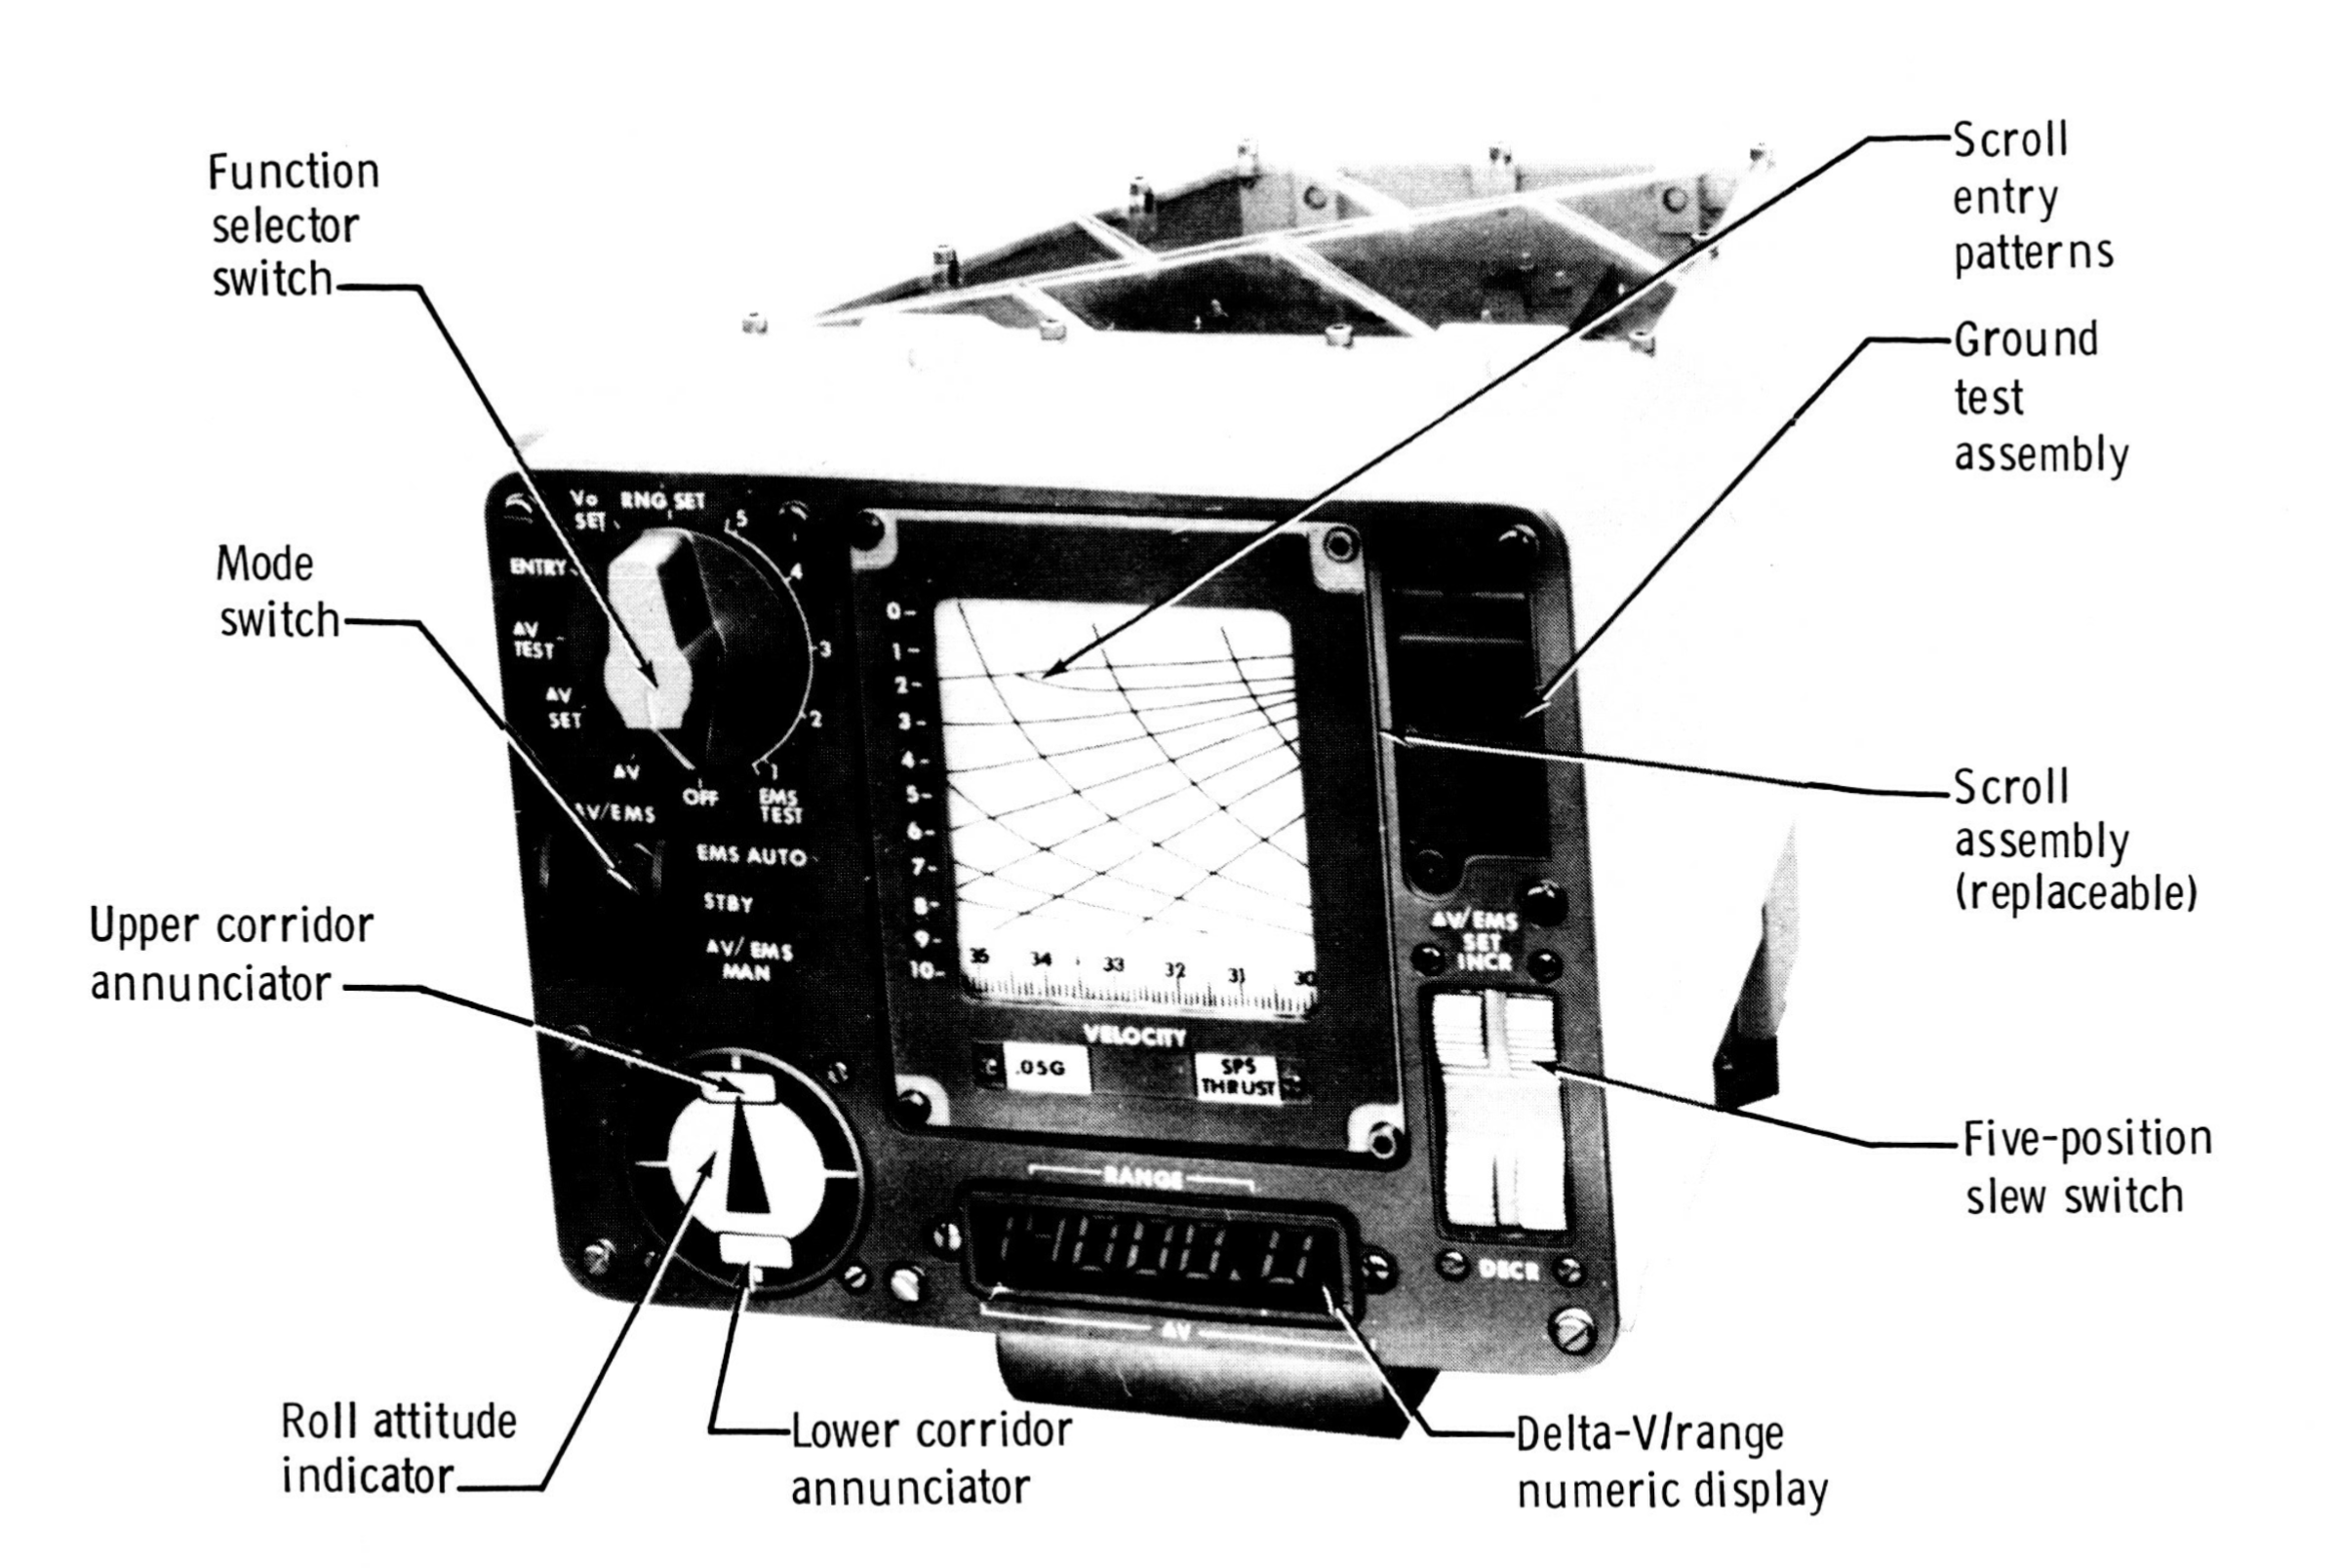
\includegraphics[width=\linewidth]{papers/leo/Grafiken/EMS.png}
	\caption{Abbildung eines EMS der Apollo-Mision, aus dem Erfahrungsbericht \cite{leo:wilson1976apollo}.}
	\label{fig:leo:ems}
\end{figure}


